% !TeX encoding = ISO-8859-1
\chapter[Related Work]{Related Work}
\label{ch:relwork}

The work of this thesis is divided into two main tasks:
\begin{itemize}
 \item \textbf{Pixelwise Semantic Segmentation}
 \item \textbf{Temporary Consistent Segmentation}
\end{itemize}

The following sections contain related work with state of the art results.

\section{Semantic Segmentation}
\label{sec:pixsemseg}
Semantic segmentation task is approached using a deep learning method, the so-called \textit{Convolutional Neural Networks}. This decision is based on the recent success of CNN models for visual tasks (e.g. image classification (\textcite{Krizhevsky_imagenetclassification} \textcite{szegedy2014going}, \textcite{simonyan2014very}), object detection (\textcite{sermanet2013overfeat},\textcite{girshick2014rich}), local correspondence (\textcite{fischer2014descriptor}, \textcite{NIPS2014_5420})) and more recently in pixelwise labeling task (\textcite{farabet2013pami}, \textcite{lin2015efficient}, \textcite{long2014fully}, \textcite{chen14semantic}, \textcite{hariharan2014hypercolumns}). 
 
Current state of the art segmentation methods are observable in the \href{http://host.robots.ox.ac.uk:8080/leaderboard/displaylb.php?challengeid=11&compid=6/}    {Pascal VOC 2012 website}. 
Most of the presented methods possess a CNN stage or are completely based on Convolutional Neural Networks. \textcite{lin2015efficient}, \textcite{chen14semantic} have reached outstanding performance and when compared with similar approaches, both show a combination of CNNs and \textit{Conditional Random Fields} (CRFs). 

All these methods are similar to \textcite{farabet2013pami}, which successfully implemented the strengths of CNNs and CRFs together. The CNNs perform especially well for feature representations, while the CRFs capture contextual relation modeling. In order to obtain a more robust feature representation, a multi-scale pyramid was added at the beginning. The multi-scale pyramid exploits different feature representations that are only seen at a certain scale. Figure ~\ref{fig:farabet} presents a diagram of the scene parsing system proposed by \textcite{farabet2013pami}. It consists of two parallel branches where the first one is composed by a Laplacian pyramid and a CNN. The latter branch is a superpixel segmentation or a segmentation tree followed by a CRF model. Both branches are merged to produce a final pixelwise classification.

\begin{figure}
 \centering
 \includegraphics[scale=0.25]{farabet}
 \caption{Scene parsing System from \textcite{farabet2013pami}}
 \label{fig:farabet}
\end{figure}   

\textcite{hong2015decoupled} and \textcite{noh2015learning} approaches differ significantly from the typical CNN models. Both propose a two CNN model, where the classification and segmentation tasks are decoupled. Each CNN deals with an independent task. This decoupled architecture offers the possibility to train CNN separately. These approaches mitigate the heavy requirement of a large number of segmentation ground truth data by using weakly-supervised learning methods. Object labels associated with an input image are identified by a classification network, and object figure ground segmentation by the segmentation network. There is a third element in this algorithm: the bridging layers. Their function is to tight the otherwise loose connections between classification and segmentation. This algorithm solves two drawbacks of traditional segmentation methods: smoothed or lost detailed structures due a coarse label map (present in end-to-end systems using only CNNs)  and a fixed-sized receptive field (no multi-scale representation), which leads to fragmented or mislabeled segmentations. Figure ~\ref{fig:hong} gives an overview of this architecture. 

\begin{figure}
 \centering
 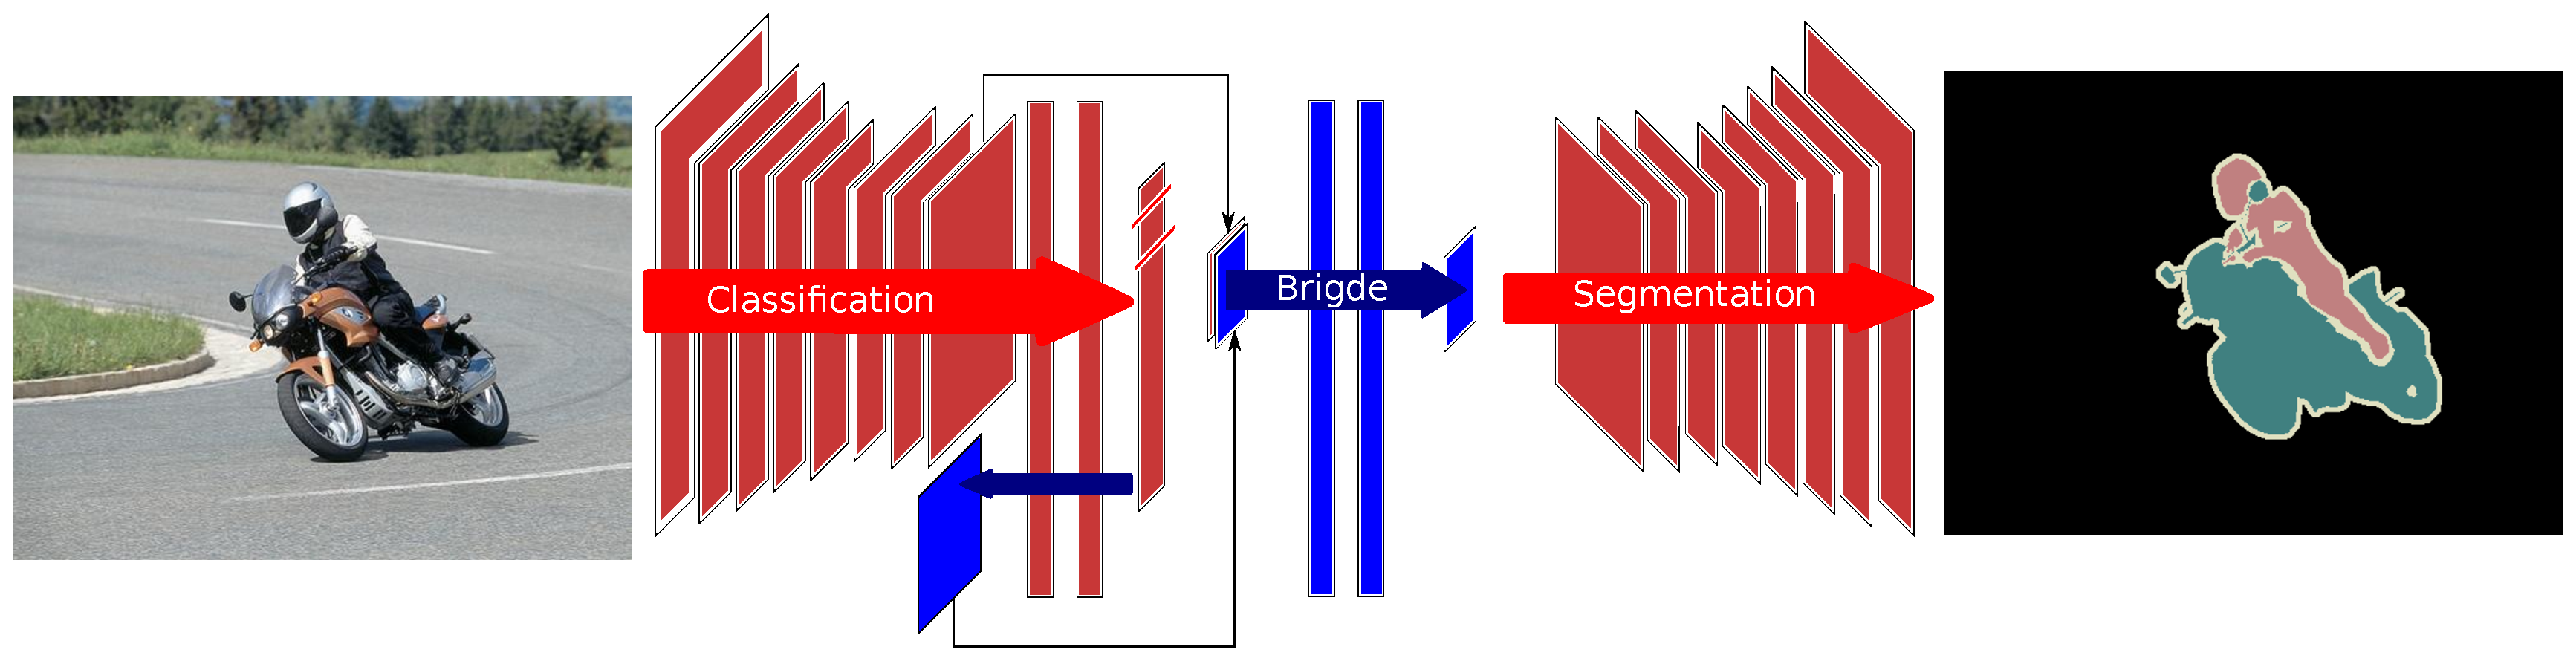
\includegraphics[scale=0.25]{hong}
 \caption{Architecture of the networks proposed in \textcite{hong2015decoupled}. Classification takes places through several convolution layers. Semantic segmentation uses deconvolutional layers to rebuild the original image.}
 \label{fig:hong}
\end{figure}
% show network architecture.

\textcite{hariharan2014hypercolumns} introduce the \textit{"Hypercolumn"} taken from neuroscience to also produce state of the art results. In order to overcome a problem with information from the last layers being too coarse, information from early layers must be also considered.  The hypercolumn allows to have information from several layers inside the CNN. It benefits from the trade-off between different layers by combining them. The last layers capture semantics in a more efficient way (category-level information), while the early layers help to obtain a more precise location (e.g. pose, illumination, articulation, location, etc.). The \textit{Hypercolumns} work as pixel descriptors, and were successfully used for diverse visual tasks (e.g. detection, segmentation, keypoint localization and part labeling).
Needless to say, it also uses multiple levels of abstraction and scale are necessary. This can be comparable to \textcite{farabet2013pami} mutli-scale pyramid.However the invariance in is similar, since the features come from the same level of the CNN. Figure ~\ref{fig:hyper} shows the hypercolumn idea implemented in a CNN. 

\begin{figure}
 \centering
 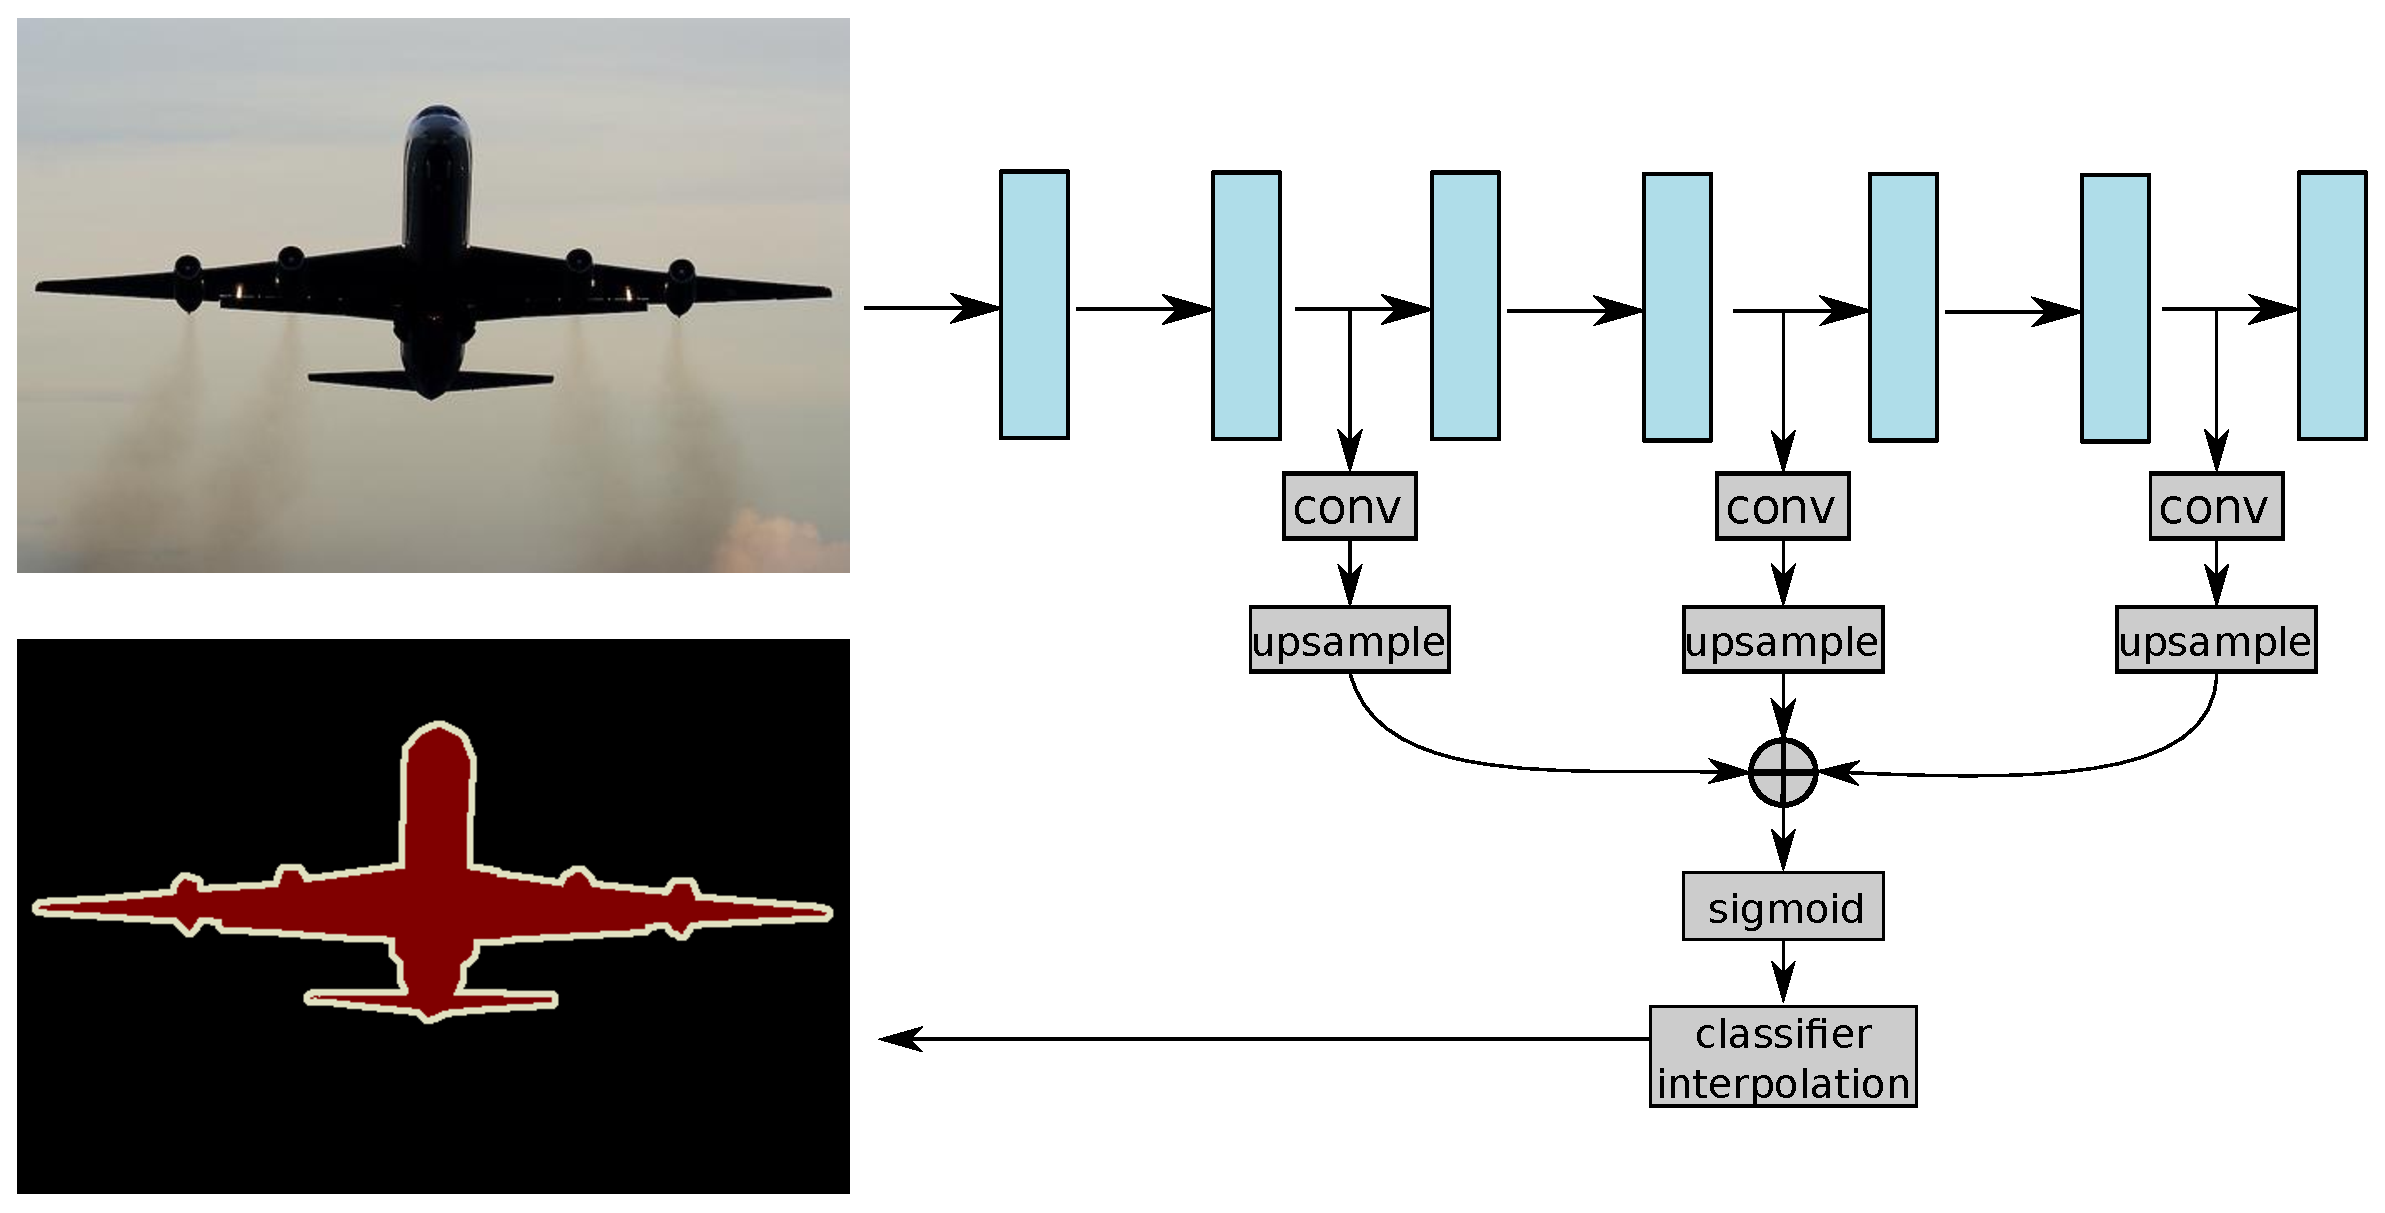
\includegraphics[scale=0.3]{hypercolumns}
 \caption{Original classification CNN is shown in blue, and added layers for the hypercolumn classifier are in gray (\textcite{hariharan2014hypercolumns}).}
 \label{fig:hyper} 
\end{figure}


Notably, \textcite{long2014fully} present an end-to-end system for semantic segmentation using only \textit{fully convolutional} networks. The models presented here are characterized for an architecture which combines deep, coarse, semantic informantion and shallow, fine, appearance information in a multi-layer framework. The fully convolutional models are obtained from  pre-trained CNN that perform image classification (\textcite{Krizhevsky_imagenetclassification}, \textcite{szegedy2014going} and \textcite{simonyan2014very}). In order to make them suitable for pixelwise classification, the inner product layers are replaced by convolutional layers, while a transfer of parameters occurs based on \textcite{donahue2013decaf}. A fine-tuning process is driven to adapt the fully convolutional networks for new semantic segmentation tasks. In order to produce finer segmentations, different layers are upsamled and fused. The main advantages of this approaches lay in the capacity of reusing learned values, reducing the need of a big training dataset (which is costly effort) and the use of Caffe. Figure ~\ref{fig:fcn} explains how semantic segmentation is possible with a fully convolutional net.

The approach of this thesis is based on \textcite{long2014fully}. Fully convolutional networks are possible to train using Caffe (\textcite{jia2014caffe}) as framework. Caffe allows to use pre-trained models, which are \href{https://github.com/BVLC/caffe/wiki/Model-Zoo}{publicly available} and well documented. It is also handy to choose this framework due the big communities of \href{https://groups.google.com/forum/#!forum/caffe-users}{users} and \href{https://github.com/BVLC/caffe}{developers}.  In order to make fine-tuning using a small dataset (\textcite{BrostowFC:PRL2008}) feasible, this thesis also makes use of transfer of parameters exposed in \textcite{donahue2013decaf}.  

\begin{figure}
 \centering
 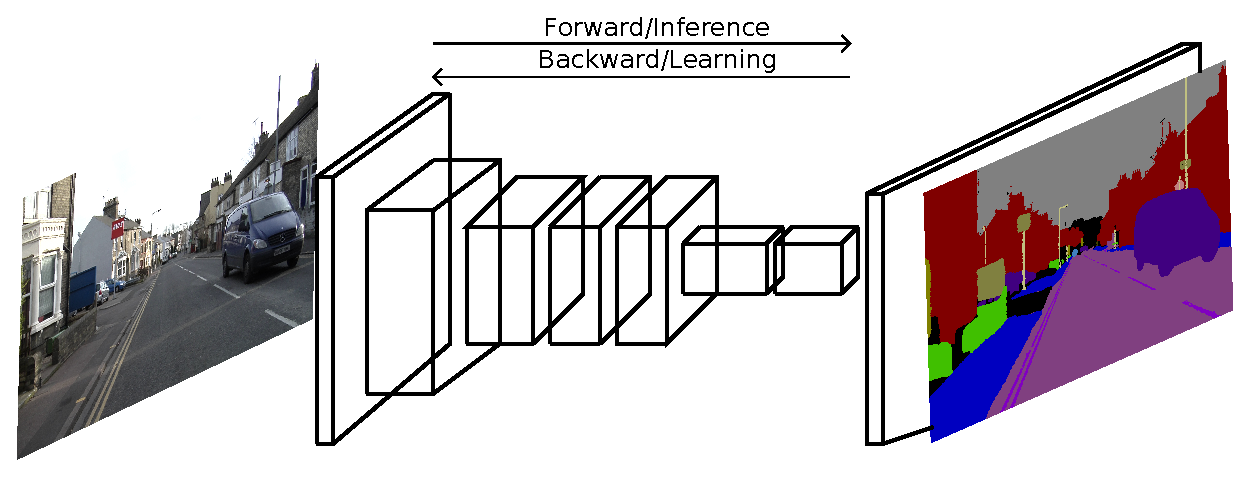
\includegraphics[scale=0.7]{camvid_convolution}
 \caption{Fully convolutional networks make dense predictions for pixel classification.The final layer makes use of a bilinear interpolation to produce the semantic segmentation}
 \label{fig:fcn}
\end{figure}
   

\section{Temporary Semantic Segmentation}
\label{sec:tempsemseg}
This section presents the approaches with state of the art results for temporary semantic segmentation. Since it is desired to yield a causal segmentation for online applications, omniscient methods are not covered due their inherent need of future frames. The purpose of this implementation is to enhance the traffic scene labeling using a temporary relation (besides the spatial relation from the CNN). The final result is expected to have avoid flickering segmentations and to increase the accuracy based on previous knowledge. Figure ~\ref{fig:causal} shows the desired kind of approach. %Add image with omniscient, causal and frame by frame.

%The taken approach is to adapt the CNN model for temporal fusion of the predicted outputs. The main idea behind such an approach is to overcome the traffic scene labeling not only by spatial relation but also using temporary relation in order to improve its performance.
 
\textcite{ess2009segmentation} is a work whose purposes are very similar to the ones from this thesis. A two-stages approach is introduced where the first stage generates a superpixel segmentation based on \textcite{felzenszwalb2004efficient}, which is later used in a second stage to construct a feature set for a classifier. The proposed image-based system is able to perform road recognition as well as a set of objects (e.g. cars, pedestrians, etc.). In order to allow online applications, the temporal smoothing is obtained using the forward pass output of a \textit{Hidden Markov Model} (HMM) \textcite{rabiner1989tutorial}.

\begin{figure}
 \centering
 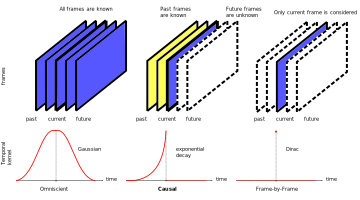
\includegraphics[scale=1.2]{segmentation_types}
 \caption{There are three types of video segmentation. In order to improve the segmentation performance, this thesis focuses on causal segmentation.}
  \label{fig:causal}
\end{figure} 

\textcite{paris2008edge} profit from the spatial-temporal dimensions mix from video datasets. This approach relies on a bilateral filtering and a mean-shift segmentation from \textcite{paris2007topological}. This is an online approach, therefore it only uses current and past data. The previously acquired data helps to ensure temporal coherence which otherwise cannot be accomplished by using frame-by-frame approaches.

\textcite{grundmann2010efficient} use a hierarchical graph-based algorithm in order to yield a temporary consistent segmentation. This algorithm addresses three problems: Temporal coherence, automatic tracking and scalability. Like similar approaches,  it is initialized with an oversegmentation using the graph-based image segmentation from \textcite{felzenszwalb2004efficient}. Afterwards, the algorithm makes use of Optical Flow (\textcite{horn1981determining}) to modify the graph structure with respect to time. A hierarchical segmentation yields a region grpah from a previous segmentation level.  This approach exhibits long-term temporal coherence and overcomes memory and runtime 

%\textcite{karpathy2014large} have successfully used CNNs to classify videos. This work denoted how it is possible to take advantage of local-tempral information within the CNNs.
\textcite{miksik2013efficient} perform a scene analysis generating predictions of semantic categories over time. These predictions are characterized for being spatially and temporally consistent. It is an online algorithm which uses a temporal filter based on exponential smoothing over past predictions. This method can be applied in combination with any frame-by-frame analysis technique, as long as it produces a pixelwise labeling. This temporally smoothing technique works using Optical Flow (\textcite{horn1981determining}) to estimate correspondances with the previous frame.
  
\textcite{couprie2014convolutional} propose an approach whose objectives are similar to the ones of this thesis. It yields real-time segmentation of indoor scenes. This method benefits from the semantic segmentation of \textcite{farabet2013pami}. In order to improve the performance of the segmentation, the temporal consistency of the video sequences is exploited. This causal segmentation is taken from \textcite{couprie2013causal} and uses the superpixel segmentation method from \textcite{felzenszwalb2004efficient}. A graph-matching technique is developed in order to match previous segmentations and to enrich the current frame segmentation. The main advantages of this approach are the computational efficiency and the possibility of future implementations working together with another frame-by-frame technique.

The method developed in this thesis, makes use of the causal segmentation proposed in \textcite{couprie2013causal}, due its capabilities for real-time implementations and the availability of the \href{http://perso.esiee.fr/~coupriec/code.html}{programming code}. 



%
%
%

